\documentclass[10pt,a4paper]{article}
\usepackage[a4paper, total={6.7in, 9in}]{geometry}
\usepackage[latin1]{inputenc}
\usepackage{amsmath}
\usepackage{amsfonts}
\usepackage{amssymb}
\usepackage{mathtools}
\usepackage{graphicx}
\usepackage{float}
\usepackage[usenames, dvipsnames]{color}
\usepackage{fancyhdr}
\usepackage{enumitem}
\usepackage{listings}
\usepackage{rotating}
\setlength{\headheight}{15.2pt}
\pagestyle{fancy}
\setlength{\parindent}{0em}
\setlength{\parskip}{10pt}
\setlist[enumerate,1]{label=\alph*)}
\setlist[enumerate,2]{label=(\roman*)}
\definecolor{LGray}{gray}{0.9}
\definecolor{DGray}{gray}{0.4}
\usepackage{inconsolata}
\usepackage[T1]{fontenc}
\lstset{language=Matlab, tabsize=2, breaklines=true, postbreak=\mbox{\textcolor{red}{$\hookrightarrow$}\space}, basicstyle=\linespread{0.7}\ttfamily, commentstyle=\color{DGray}} 
\newcommand*\diff{\mathop{}\!\mathrm{d}}



\begin{document}
\title{ENGSCI762 A2}
\author{Benjamin Yi}
\rhead{Benjamin Yi - byi649 - 925302651}
\lhead{ENGSCI762 A2}
	
\section*{Question 1}
Ordering: shortest weighted processing time first.

Proof: \\
Let \(i(1)\) be the first job processed, \(i(2)\) the second etc\\
With shortest weighted processing time we have:\\
\begin{equation*}
	w_1p_{i(1)} \leq w_2p_{i(2)} \leq \dots \leq w_np_{i(n)}
\end{equation*}
Now consider some order with 
\begin{equation}\label{contra}
	w_kp_{i(k)} \geq w_{k+1}p_{i(k+1)}
\end{equation}
Let job \(i(k-1)\) be completed at time \(t\), then:
\begin{align*}
	C_{i(k)} &= t + p_{i(k)}\\
	C_{i(k+1)} &= t + p_{i(k)} + p_{i(k+1)}\\
	\sum_i^n w_iC_i &= \sum_{\substack{j=1\\j \ne k, j \ne k+1}}^n w_jC_{i(j)} + w_kC_{i(k)} + w_{k+1}C_{i(k+1)}
\end{align*}
The objective function becomes:
\begin{equation*}
	z_1 =  \sum_{\substack{j=1\\j \ne k, j \ne k+1}}^n w_jC_{i(j)} + w_k(t + p_{i(k)}) + w_{k+1}(t + p_{i(k)} + p_{i(k+1)})
\end{equation*}
Now swap job order of \(i(k), i(k+1)\):
\begin{equation*}
	z_2 =  \sum_{\substack{j=1\\j \ne k, j \ne k+1}}^n w_jC_{i(j)} + w_{k+1}(t + p_{i(k+1)}) + w_k(t + p_{i(k)} + p_{i(k+1)})
\end{equation*}
The change in objective function becomes:
\begin{align*}
	z_2 - z_1 &= w_{k+1}(t + p_{i(k+1)}) + w_k(t + p_{i(k)} + p_{i(k+1)}) - w_k(t + p_{i(k)}) - w_{k+1}(t + p_{i(k)} + p_{i(k+1)})\\
	&= w_kp_{i(k+1)} - w_{k+1}p_{i(k)}\\
	&= w_{k+1}p_{i(k+1)}\bigg[\frac{w_k}{w_{k+1}} - \frac{p_{i(k)}}{p_{i(k+1)}}\bigg]
\end{align*}
From (\ref{contra}), knowing weights and processing times are positive, we can state:
\begin{equation*}
	\frac{p_{i(k+1)}}{p_{i(k)}} \geq \frac{w_k}{w_{k+1}}
\end{equation*}
Therefore \(z_2 - z_1 \leq 0\), meaning switching to shortest weighted processing time order can only improve or maintain the solution.  This proves shortest weighted processing time order is optimal.\\
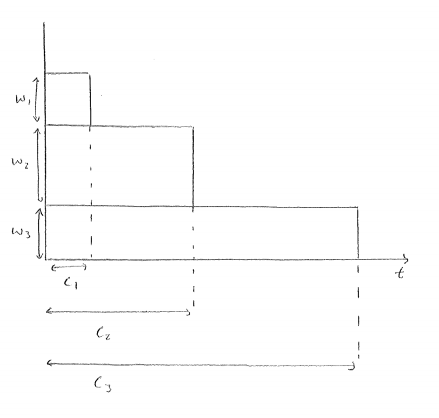
\includegraphics[width=0.7\linewidth]{q1}
\section*{Question 2}
\begin{enumerate}
	\item \text{}\\
	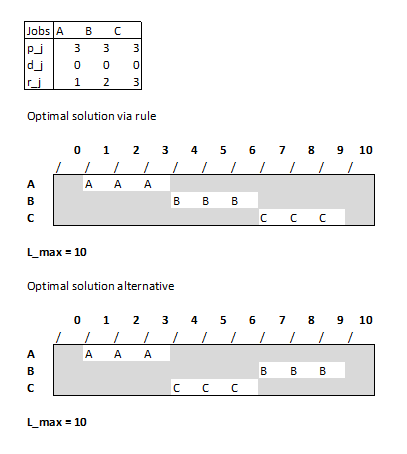
\includegraphics[width=0.7\linewidth]{q2}

	
	\item 1/\(r_j\)/\(C_\text{max}\)
\end{enumerate}

\section*{Question 3}
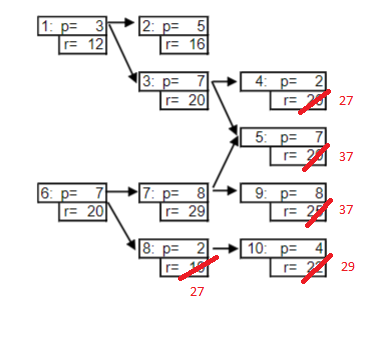
\includegraphics[width=0.7\linewidth]{q3}\\
Maximum lateness = 21\\
Order: 1, 2, 3, 6, 4, 8, 7, 10, 5, 9
\newpage	
\begin{sidewaysfigure}
	\centering
	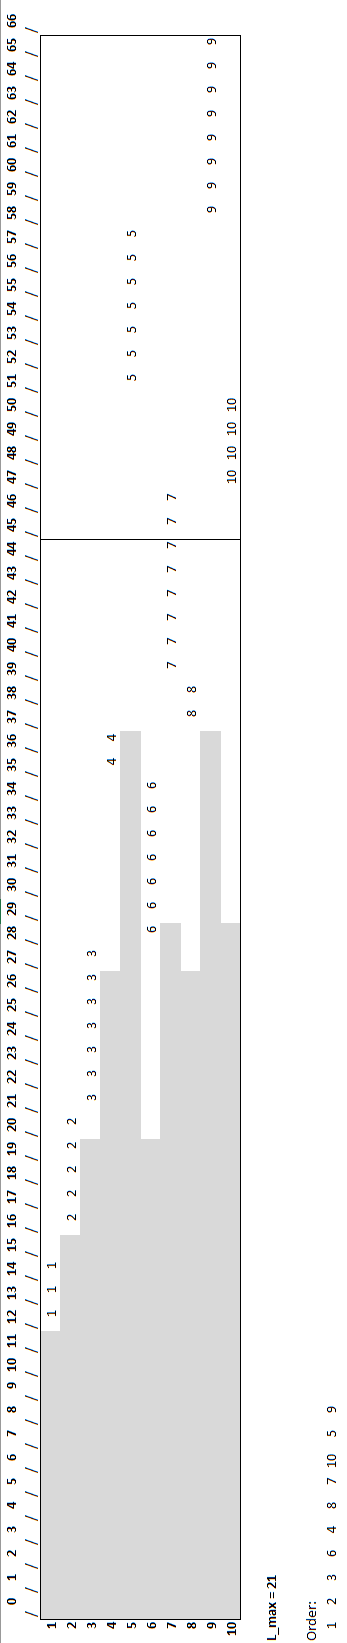
\includegraphics[width=1\linewidth]{q3_2}
\end{sidewaysfigure}

\end{document}

